\documentclass[dvipdfmx]{jsarticle}
\usepackage[final]{graphicx}
\usepackage{float} % 追加: floatパッケージのインクルード
% 数式
\usepackage{amsmath,amsfonts}
\usepackage{bm}
% 画像
% \lstset{noxoutput=true}

\include{setting.txt}


\begin{document}

\title{キューの作成} 
\author{22060 211 古城隆人}
\date{\today}
\maketitle

% \tableofcontents

\newpage


\section{目的}
キューのデータ構造を理解し、実装することで、キューの基本的な動作を理解する。キューを実装する方法として配列、リングバッファ、リスト構造を用いて実装を行う。
リスト構造ではメモリの確保と解放を行うので、メモリの確保と解放の方法の理解も目的とする。
\section{原理}
\subsection{キュー}
キューは、データを先入れ先出し(FIFO)で処理するデータ構造である。キューは、データを追加するenqueueとデータを取り出すdequeueの2つの操作を持つ。
enqueueはキューの末尾にデータを追加し、dequeueはキューの先頭からデータを取り出す。キューは、配列、リングバッファ、リスト構造を用いて実装することができる。
\subsection{配列}
配列を用いてキューを実装する場合、配列の先頭をキューの先頭とし、末尾をキューの末尾とする。enqueueは末尾にデータを追加し、dequeueは先頭からデータを取り出す。
でキューされるたびに配列の要素をずらすため、演算にかかる時間が長くなる。
\subsection{リングバッファ}
リングバッファを用いてキューを実装する場合、配列の先頭と末尾をつなげて演算を行う。また、キューの先頭と配列のインデックスの数を格納するための変数も用意する。
この方法では、配列の要素をずらすことなくキューを実装することができる。
データ構造を\ref{lst:queueh}に示す。
\begin{lstlisting}[caption={queue.h}, label={lst:queueh}]
#define QUEUE_SIZE 5
struct queue
{
    int array[QUEUE_SIZE]; // データが入る配列
    int wp;                // 次にデータを入れる場所の配列番号
    int quantity;          // データの個数
};
\end{lstlisting}
\subsection{リスト構造}
リスト構造を用いてキューを実装する場合、メモリの確保を行ってデータを格納する。
リスト構造は、データを格納するための構造体と次のデータを指すポインタを持つ。データ構造を\ref{lst:queueh}に示す。
\begin{lstlisting}[caption={queue.h}, label={lst:queueh}]
struct queue
{
    int val;
    struct queue *addr;
};
struct queue *bottom_queue = NULL; // 最古のキューのアドレスを記憶しておくポインタ
struct queue *top_queue = NULL;    // 最新のキューのアドレスを記憶しておくポインタ
\end{lstlisting}
プログラムのコメントアウトにもあるが、bottom\_queueは最古のキューのアドレスを記憶しておくポインタであり、top\_queueは最新のキューのアドレスを記憶しておくポインタである。
\section{実験環境}
実験環境を表\ref{tab:environment}に示す。
\begin{table}[ht]
  \centering
  \begin{tabular}{|c|c|}
    \hline
    \textbf{項目} & \textbf{値}              \\
    \hline
    OS          & windows10上のwsl2(Ubuntu) \\
    \hline
    CPU         & Intel Core i7 11800H          \\
    \hline
    メモリ         & 8GB                     \\
    \hline
    コンパイラ       & gcc 11.4.0              \\
    \hline
  \end{tabular}
  \caption{実験環境}
  \label{tab:environment}
\end{table}
\section{プログラムの設計と説明}
\subsection{配列を用いたキューの実装}
配列を用いてキューを作成するために関数の作成を行う。
\subsubsection{作成した関数}
\textbf{・enqueue関数}\\
このプログラムでは、配列にキューを追加する。配列はグローバル変数と宣言しているため引数はキューに追加するでーただけである。
\begin{table}[ht]
  \centering
  \caption{enqueue関数}
  \begin{tabular}{|p{5cm}|p{10cm}|}
    \hline
    機能  & キューにデータを追加する。                                      \\
    \hline
    引数  & int data : 追加するデータ \\
    \hline
    戻り値 & int : エラーコード(-100:正常終了, -101:キューが満杯, -102:データが自然数でない) \\
    \hline
  \end{tabular}
  \label{tab:enqueue_func}
\end{table}
\begin{lstlisting}[caption={enqueue関数}, label={lst:enqueue_func}]
int enqueue(int data)
{
    // 残り領域があるか確認する
    if (quantity >= QUEUE_SIZE)
    {
        return -101;
    }
    // データが自然数か確認する
    if (data < 0)
    {
        return -102;
    }
    // 配列のキューにデータを保存する
    queue[quantity] = data;
    // キューのポインタをインクリメントする
    quantity++;
    // 返り値を返す
    return -100;
}
\end{lstlisting}
\textbf{・dequeue関数}\\
このプログラムでは、配列からキューを取り出す。配列はグローバル変数と宣言しているため引数はない。返り値として取り出したデータを返す。
\begin{table}[ht]
  \centering
  \caption{dequeue関数}
  \begin{tabular}{|p{5cm}|p{10cm}|}
    \hline
    機能  & キューからデータを取り出す。                                      \\
    \hline
    引数  & なし \\
    \hline
    戻り値 & int : エラーコード(-201:データが存在しない, データ:正常終了) \\
    \hline
  \end{tabular}
  \label{tab:dequeue_func}
\end{table}
\begin{lstlisting}[caption={dequeue関数}, label={lst:dequeue_func}]
int dequeue(void)
{
    // データが存在するかどうか確認する.
    if (quantity <= 0)
    {
        return -201;
    }
    // キューからデータをとりだす.
    int data = queue[0];
    // データの個数カウントを減らす
    quantity--;
    // 取り出されたデータ部分を埋めるように再構築する
    for (int i = 0; i < quantity; i++)
    {
        queue[i] = queue[i + 1];
    }
    // 空き領域を初期化する.
    queue[quantity] = 0;
    // データもしくは返り値を返す
    return data;
}
\end{lstlisting}
\textbf{・initQueue関数}\\
このプログラムでは、配列を初期化する。配列はグローバル変数と宣言しているため引数はない。配列の中身をすべて0にすることで初期化を行う。
\begin{table}[ht]
  \centering
  \caption{initQueue関数}
  \begin{tabular}{|p{5cm}|p{10cm}|}
    \hline
    機能  & キューを初期化する。                                      \\
    \hline
    引数  & なし \\
    \hline
    戻り値 & int : エラーコード(0:正常終了) \\
    \hline
  \end{tabular}
  \label{tab:initQueue_func}
\end{table}
\begin{lstlisting}[caption={initQueue関数}, label={lst:initQueue_func}]
int initQueue()
{
    // キューのデータを入れる配列をすべて 0 に初期化する.
    for (int i = 0; i < QUEUE_SIZE; i++)
    {
        queue[i] = 0;
    }
    // 格納データ個数を 0 に初期化する.
    quantity = 0;
    return 0;
}
\end{lstlisting}
\textbf{・showQueue関数}\\
このプログラムでは、配列の中身を表示する。配列はグローバル変数と宣言しているため引数はない。配列の中身をすべて表示する。
\begin{table}[ht]
  \centering
  \caption{showQueue関数}
  \begin{tabular}{|p{5cm}|p{10cm}|}
    \hline
    機能  & キューの中身を表示する。                                      \\
    \hline
    引数  & なし \\
    \hline
    戻り値 & int : エラーコード(0:正常終了) \\
    \hline
  \end{tabular}
  \label{tab:showQueue_func}
\end{table}
\begin{lstlisting}[caption={showQueue関数}, label={lst:showQueue_func}]
int showQueue()
{
    // 配列全体のデータを順に表示する.
    // データとデータの間に区切り文字「|」を表示する.
    for (int i = 0; i < QUEUE_SIZE; i++)
    {
        printf("%d|", queue[i]);
    }
    return 0;
}
\end{lstlisting}
\textbf{・showResult関数}\\
このプログラムでは、エラーコードに応じてエラーメッセージを表示する。引数としてエラーコードを受け取り、エラーコードに応じたエラーメッセージを表示する。
\begin{table}[ht]
  \centering
  \caption{showResult関数}
  \begin{tabular}{|p{5cm}|p{10cm}|}
    \hline
    機能  & 関数の実行結果を表示する。                                      \\
    \hline
    引数  & int result : エラーコード \\
    \hline
    戻り値 & なし \\
    \hline
  \end{tabular}
  \label{tab:showResult_func}
\end{table}
\begin{lstlisting}[caption={showResult関数}, label={lst:showResult_func}]
  void showResult(int result)
{
    // result の値に応じて,対応するエラーメッセージを表示する.
    showQueue();
    printf("--> %d:", result);
    switch (result)
    {
    case -100:
        printf("enqueue 成功\n");
        break;
    case -101:
        printf("エラー:キューが満杯です\n");
        break;
    case -102:
        printf("エラー:データが自然数ではありません\n");
        break;
    case -201:
        printf("エラー:キューが空です\n");
        break;
    default:
        if (result < 0)
        {
            printf("エラー:不明なエラーです\n");
        }
        else
        {
            printf("dequeue(%d)\n", result);
        }
        break;
    }
}
\end{lstlisting}
\textbf{・main関数}\\
キューが正しく動作しているかを確かめるためにmain関数を作成する。main関数はキューの初期化、enqueue、dequeue、showQueue、showResultを行う。
キューをあふれさせるために5回enqueueを行っている。また、キューが空かどうかの判定ができているかを確かめるために5回dequeueを行っている。
グローバル変数として定義している配列は、インデックスが4個しかないため5回操作を行うとエラーが出てくるはずである。
\begin{lstlisting}[caption={main関数}, label={lst:main_func}]
int main()
{
    // キューを初期化する
    initQueue();
    // キューにデータを追加する
    showResult(enqueue(1));
    showResult(enqueue(2));
    showResult(enqueue(3));
    showResult(enqueue(4));
    showResult(enqueue(5));
    // キューの中身を表示する
    // showQueue();
    // キューからデータを取り出す
    showResult(dequeue());
    showResult(dequeue());
    showResult(dequeue());
    showResult(dequeue());
    showResult(dequeue());
    // キューの中身を表示する
    // showQueue();
    return 0;
}
\end{lstlisting}
\subsection{リングバッファを用いたキューの実装}
リングバッファを用いてキューを作成するために関数の作成を行う。
\subsubsection{作成した関数}
\textbf{・enqueue関数}\\
このプログラムでは、リングバッファにキューを追加する。リングバッファは構造体で宣言しているため引数は構造体と追加するデータである。
\begin{table}[ht]
  \centering
  \caption{enqueue関数}
  \begin{tabular}{|p{5cm}|p{10cm}|}
    \hline
    機能  & キューにデータを追加する。                                      \\
    \hline
    引数  & struct queue *obj : キューの構造体, int data : 追加するデータ \\
    \hline
    戻り値 & int : エラーコード(-100:正常終了, -101:キューが満杯, -102:データが自然数でない) \\
    \hline
  \end{tabular}
  \label{tab:enqueue_func_2}
\end{table}
\newpage
\begin{lstlisting}[caption={enqueue関数}, label={lst:enqueue_func_2}]
int enqueue(struct queue *obj, int data)
{
    // 残り領域があるか確認する.
    // データが自然数か確認する.
    // 配列にデータを保存する.
    // 最新のデータが入った場所の次の場所を指すように値を更新する.
    // データの個数カウントを増やす.
    // 返り値を返す.
    if (obj->quantity >= QUEUE_SIZE)
    {
        return -101;
    }
    if (data < 0)
    {
        return -102;
    }
    obj->array[obj->wp] = data;
    obj->wp = (obj->wp + 1) % QUEUE_SIZE;
    obj->quantity++;
    return -100;
}
\end{lstlisting}
\textbf{・dequeue関数}\\
このプログラムでは、リングバッファからキューを取り出す。リングバッファは構造体で宣言しているため引数は構造体である。
\begin{table}[ht]
  \centering
  \caption{dequeue関数}
  \begin{tabular}{|p{5cm}|p{10cm}|}
    \hline
    機能  & キューからデータを取り出す。                                      \\
    \hline
    引数  & struct queue *obj : キューの構造体 \\
    \hline
    戻り値 & int : エラーコード(-201:データが存在しない, データ:正常終了) \\
    \hline
  \end{tabular}
  \label{tab:dequeue_func_2}
\end{table}
\begin{lstlisting}[caption={dequeue関数}, label={lst:dequeue_func_2}]
int dequeue(struct queue *obj)
{
    // データが存在するかどうか確認する.
    // キューからデータをとりだす.
    // データの個数のカウントを減らす.
    // データもしくは返り値を返す.
    if (obj->quantity <= 0)
    {
        return -201;
    }
    int data = obj->array[0];
    obj->quantity--;
    obj->array[(obj->wp+QUEUE_SIZE - obj->quantity - 1) % QUEUE_SIZE] = 0;
    return data;
}
\end{lstlisting}
\textbf{・initQueue関数}\\
このプログラムでは、リングバッファを初期化する。リングバッファは構造体で宣言しているため引数は構造体である。
\begin{table}[ht]
  \centering
  \caption{initQueue関数}
  \begin{tabular}{|p{5cm}|p{10cm}|}
    \hline
    機能  & キューを初期化する。                                      \\
    \hline
    引数  & struct queue *obj : キューの構造体 \\
    \hline
    戻り値 & int : エラーコード(0:正常終了) \\
    \hline
  \end{tabular}
  \label{tab:initQueue_func_2}
\end{table}
\begin{lstlisting}[caption={initQueue関数}, label={lst:initQueue_func_2}]
int initqueue(struct queue *obj)
{
    // キューのデータを入れる配列をすべて 0 に初期化する.
    // キューのデータ格納個数を 0 に初期化する
    // キューの wp ポインタを 0 に初期化する.
    for (int i = 0; i < QUEUE_SIZE; i++)
    {
        obj->array[i] = 0;
    }
    obj->quantity = 0;
    obj->wp = 0;
    return 0;
}
\end{lstlisting}
\textbf{・showQueue関数}\\
このプログラムでは、リングバッファの中身を表示する。リングバッファは構造体で宣言しているため引数は構造体である。
\begin{table}[ht]
  \centering
  \caption{showQueue関数}
  \begin{tabular}{|p{5cm}|p{10cm}|}
    \hline
    機能  & キューの中身を表示する。                                      \\
    \hline
    引数  & struct queue *obj : キューの構造体 \\
    \hline
    戻り値 & int : エラーコード(0:正常終了) \\
    \hline
  \end{tabular}
  \label{tab:showQueue_func_2}
\end{table}
\begin{lstlisting}[caption={showQueue関数}, label={lst:showQueue_func_2}]
int showQueue(struct queue *obj)
{
    // 配列全体のデータを順に表示する.
    // データとデータの間に区切り文字「|」を表示する.
    for (int i = 0; i < QUEUE_SIZE; i++)
    {
        printf("%d", obj->array[i]);
        if (i < QUEUE_SIZE - 1)
        {
            printf("|");
        }
    }
    return 0;
}
\end{lstlisting}
\textbf{・showResult関数}\\
このプログラムでは、エラーコードに応じてエラーメッセージを表示する。引数としてエラーコードを受け取り、エラーコードに応じたエラーメッセージを表示する。
\begin{table}[ht]
  \centering
  \caption{showResult関数}
  \begin{tabular}{|p{5cm}|p{10cm}|}
    \hline
    機能  & 関数の実行結果を表示する。                                      \\
    \hline
    引数  & int result : エラーコード \\
    \hline
    戻り値 & なし \\
    \hline
  \end{tabular}
  \label{tab:showResult_func_2}
\end{table}
\begin{lstlisting}[caption={showResult関数}, label={lst:showResult_func_2}]
void showResult(int result)
{
    // result の値に応じて,対応するエラーメッセージを表示する.
    switch (result)
    {
    case -100:
        printf("正常終了\n");
        break;
    case -101:

        printf("エラー:キューが満杯です\n");
        break;
    case -102:
        printf("エラー:データが自然数ではありません\n");
        break;
    case -201:
        printf("エラー:キューが空です\n");
        break;
    default:
        printf("\n");
        break;
    }
}

\end{lstlisting}
\textbf{・main関数}\\
キューが正しく動作しているかを確かめるためにmain関数を作成する。main関数はキューの初期化、enqueue、dequeue、showQueue、showResultを行う。
キューをあふれさせるために6回enqueueを行っている。また、キューが空かどうかの判定ができているかを確かめるために6回dequeueを行っている。
定義にて配列の数を5個としているため、6回目のenqueueでエラーが出力されるはずである。
\begin{lstlisting}[caption={main関数}, label={lst:main_func_2}]
#define QUEUE_SIZE 5
int main(void)
{
    struct queue obj;
    int result;
    result = enqueue(&obj,40);
    initqueue(&obj);
    showQueue(&obj);
    printf("<40");
    showResult(result);
    result = enqueue(&obj,60);
    showQueue(&obj);
    printf("<60");
    showResult(result);
    result = enqueue(&obj,10);
    showQueue(&obj);
    printf("<10");
    showResult(result);
    result = enqueue(&obj,80);
    showQueue(&obj);
    printf("<80");
    showResult(result);
    result = enqueue(&obj,30);
    showQueue(&obj);
    printf("<30");
    showResult(result);
    result = enqueue(&obj,50);
    showQueue(&obj);
    printf("<50");
    showResult(result);
    result = dequeue(&obj);
    showQueue(&obj);
    printf(">%d", result);
    showResult(result);
    result = enqueue(&obj,1);
    showQueue(&obj);
    printf("<1");
    showResult(result);
    result = enqueue(&obj,2);
    showQueue(&obj);
    printf("<2");
    showResult(result);
    result = dequeue(&obj);
    showQueue(&obj);
    printf(">%d", result);
    showResult(result);
    result = dequeue(&obj);
    showQueue(&obj);
    printf(">%d", result);
    showResult(result);
    result = dequeue(&obj);
    showQueue(&obj);
    printf(">%d", result);
    showResult(result);
    result = dequeue(&obj);
    showQueue(&obj);
    printf(">%d", result);
    showResult(result);
    result = dequeue(&obj);
    showQueue(&obj);
    printf(">%d", result);
    showResult(result);
    result = dequeue(&obj);
    showQueue(&obj);
    printf(">%d", result);
    showResult(result);
    result = dequeue(&obj);
    showQueue(&obj);
    printf(">%d", result);
    showResult(result);
    result = dequeue(&obj);
    showQueue(&obj);
    printf(">%d", result);
    showResult(result);
    result = enqueue(&obj,200);
    showQueue(&obj);
    printf("<200");
    showResult(result);
    result = enqueue(&obj,300);
    showQueue(&obj);
    printf("<300");
    showResult(result);
    result = enqueue(&obj,-400);
    showQueue(&obj);
    printf("<-400");
    showResult(result);
    result = enqueue(&obj,500);
    showQueue(&obj);
    printf("<500");
    showResult(result);
    return 0;
}
\end{lstlisting}
\subsection{リスト構造を用いたキューの実装}
リスト構造を用いてキューを作成するために関数の作成を行う。
\subsubsection{作成した関数}
\textbf{・enqueue関数}\\
このプログラムでは、リスト構造にキューを追加する。構造体はグローバル変数で宣言しているため、引数は追加するデータのみである。
\begin{table}[ht]
  \centering
  \caption{enqueue関数}
  \begin{tabular}{|p{5cm}|p{10cm}|}
    \hline
    機能  & キューにデータを追加する。                                      \\
    \hline
    引数  & int data : 追加するデータ \\
    \hline
    戻り値 & int : エラーコード(-100:正常終了, -101:メモリの確保ができない, -102:データが自然数でない) \\
    \hline
  \end{tabular}
  \label{tab:enqueue_func_3}
\end{table}
\begin{lstlisting}[caption={enqueue関数}, label={lst:enqueue_func_3}]
int enqueue(int data)
{
    int r_val = -100;                            // 返り値を宣言する
    struct queue *new_queue;                     // 新しく確保する領域(構造体)へのポインタを宣言する
    if (data < 0 /*挿入するデータが 0 以下であったとき*/) // 0 以下のデータが入力された時
    {
        r_val = -102; // 返り値を設定する
    }
    // 追加する領域を確保する
    /*malloc で構造体のオブジェクトの領域を確保して,確保失敗した時*/
    else if ((new_queue = (struct queue *)malloc(sizeof(struct queue))) == NULL)
    {
        // 確保できなかったとき
        r_val = -101;
    }
    else
    {
        // 新しいキューのデータ値として引数のデータを入れる(enqueue:2-1)
        new_queue->val = data;
        // 新しいキューのアドレス値として NULL を入れる(enqueue:2-2)
        new_queue->addr = NULL;
        // まだ 1 個のキューもない時
        if (bottom_queue == NULL)
        {
            // 新しいキューが最古であるので,最古のキューを指すアドレスを更新する(enqueue:4-1)
            bottom_queue = new_queue;
            // 新しいキューが最新であるので,最新のキューを指すアドレスを更新する(enqueue:4-2)
            top_queue = new_queue;
        }
        // 1 個以上のキューがあるとき
        else
        {
            // これまで最新だった領域に新しい領域を連結する(enqueue:3-1)
            top_queue->addr = new_queue;
            // 新しい領域が最新であるので,最新を指すアドレスに代入する(enqueue:3-2)
            top_queue = new_queue;

        }
        r_val = 0;
    }

    return r_val;
}
\end{lstlisting}
\textbf{・dequeue関数}\\
このプログラムでは、リスト構造からキューを取り出す。構造体はグローバル変数で宣言しているため引数はない。
\begin{table}[ht]
  \centering
  \caption{dequeue関数}
  \begin{tabular}{|p{5cm}|p{10cm}|}
    \hline
    機能  & キューからデータを取り出す。                                      \\
    \hline
    引数  & なし \\
    \hline
    戻り値 & int : エラーコード(-200:正常終了, -201:データが存在しない, -202:予測しえないエラー) \\
    \hline
  \end{tabular}
  \label{tab:dequeue_func_3}
\end{table}
\begin{lstlisting}[caption={dequeue関数}, label={lst:dequeue_func_3}]
int dequeue()
{
    int r_val = -200;         // 返り値を入れる変数を確保する
    struct queue *new_bottom; // 新たに最古になる領域を指すポインタを宣言する
    // 残りキューが 1 個の場合
    if (top_queue == bottom_queue && bottom_queue != NULL)
    {
        // 最古のデータを返り値にするために取り出す(dequeue:1-1)
        // データを取り出した後のキューを解放する(dequeue:1-2)
        // 最新のキューがないことを宣言する(dequeue:1-3)
        // 最古のキューがないことを宣言する(dequeue:1-4)
        r_val = bottom_queue->val;
        free(bottom_queue);
        top_queue = NULL;
        bottom_queue = NULL;
        
    }
    // 残りのキューが 2 個以上の場合
    else if (top_queue != NULL && bottom_queue != NULL)
    {
        // 最古のデータを返り値にするために取り出す(dequeue:2-1)
        // 新たに最古になるキューのアドレスを覚えておく(dequeue:2-2)
        // データを取り出した後のキューを解放する(dequeue:2-3)
        // 新たに最古のキューになるアドレスを更新する(dequeue:2-4)
        r_val = bottom_queue->val;
        new_bottom = bottom_queue->addr;
        free(bottom_queue);
        bottom_queue = new_bottom;
    }
    // キューが既に空っぽの場合
    else if (bottom_queue == NULL)
    {
        r_val = -201;
    }
    // 予測しえないエラー
    else
    {
        r_val = -202;
    }
    return r_val;
}
\end{lstlisting}
\textbf{・showQueue関数}\\
このプログラムでは、リスト構造の中身を表示する。構造体はグローバル変数で宣言しているため引数はない。
\begin{table}[ht]
  \centering
  \caption{showQueue関数}
  \begin{tabular}{|p{5cm}|p{10cm}|}
    \hline
    機能  & キューの中身を表示する。                                      \\
    \hline
    引数  & なし \\
    \hline
    戻り値 & int : エラーコード(0:正常終了) \\
    \hline
  \end{tabular}
  \label{tab:showQueue_func_3}
\end{table}
\begin{lstlisting}[caption={showQueue関数}, label={lst:showQueue_func_3}]
  int showQueue()
  {
      // リスト全体のデータを順に表示する.
      // データとデータの間に区切り文字「|」を表示する.
      struct queue *this_queue = bottom_queue;
      while (this_queue != NULL)
      {
          printf("%d|", this_queue->val);
          this_queue = this_queue->addr;
      }
  }
\end{lstlisting}  
\textbf{・showResult関数}\\
このプログラムでは、エラーコードに応じてエラーメッセージを表示する。引数としてエラーコードを受け取り、エラーコードに応じたエラーメッセージを表示する。
\begin{table}[ht]
  \centering
  \caption{showResult関数}
  \begin{tabular}{|p{5cm}|p{10cm}|}
    \hline
    機能  & 関数の実行結果を表示する。                                      \\
    \hline
    引数  & int result : エラーコード \\
    \hline
    戻り値 & なし \\
    \hline
  \end{tabular}
  \label{tab:showResult_func_3}
\end{table}
\begin{lstlisting}[caption={showResult関数}, label={lst:showResult_func_3}]
  void showResult(int result)
  {
      // result の値に応じて,対応するエラーメッセージを表示する.
      switch (result)
      {
      case -100:
          printf("エラー:挿入するデータが 0 以下です.\n");
          break;
      case -101:
          printf("エラー:メモリの確保に失敗しました.\n");
          break;
      case -102:
          printf("エラー:挿入するデータが 0 以下です.\n");
          break;
      case -200:
          printf("エラー:キューが空です.\n");
          break;
      case -201:
          printf("エラー:キューが空です.\n");
          break;
      case -202:
          printf("エラー:予期しないエラーが発生しました.\n");
          break;
      default:
          printf("\n");
          break;
      }
  }
\end{lstlisting}  
\newpage
\textbf{・freeQueue関数}\\
このプログラムでは、bottom\_queueのアドレスにあるメモリを開放する関数である。
\begin{table}[ht]
  \centering
  \caption{freeQueue関数}
  \begin{tabular}{|p{5cm}|p{10cm}|}
    \hline
    機能  & キューのメモリを解放する。                                      \\
    \hline
    引数  & なし \\
    \hline
    戻り値 & なし \\
    \hline
  \end{tabular}
  \label{tab:freeQueue_func}
\end{table}
\begin{lstlisting}[caption={freeQueue関数}, label={lst:freeQueue_func}]
  void freeQueue()
{
    struct queue *this_queue;
    while (bottom_queue != NULL)
    {
        // 今回開放したいキューのアドレスを取得
        // 解放後に最古になるキューのアドレスを更新
        // キューの領域を解放する
        this_queue = bottom_queue;
        bottom_queue = bottom_queue->addr;
        free(this_queue);
    }
}
\end{lstlisting}
\textbf{・main関数}\\
キューが正しく動作しているかを確かめるためにmain関数を作成する。main関数はキューの初期化、enqueue、dequeue、showQueue、showResultを行う。
リスト構造ではメモリがあふれるまでデータを追加できるため、enqueueのエラーは自然数以外が代入されたとき以外である。
\begin{lstlisting}[caption={main関数}, label={lst:main_func_3}]
int main()
{
    int result;
    result = enqueue(40);
    showQueue();
    printf("<40");
    showResult(result);
    result = enqueue(60);
    showQueue();
    printf("<60");
    showResult(result);
    result = enqueue(10);
    showQueue();
    printf("<10");
    showResult(result);
    result = enqueue(80);
    showQueue();
    printf("<80");
    showResult(result);
    result = enqueue(30);
    showQueue();
    printf("<30");
    showResult(result);
    result = enqueue(50);
    showQueue();
    printf("<50");
    showResult(result);
    result = dequeue();
    showQueue();
    printf(">%d", result);
    showResult(result);
    result = enqueue(1);
    showQueue();
    printf("<1");
    showResult(result);
    result = enqueue(2);
    showQueue();
    printf("<2");
    showResult(result);
    result = dequeue();
    showQueue();
    printf(">%d", result);
    showResult(result);
    result = dequeue();
    showQueue();
    printf(">%d", result);
    showResult(result);
    result = dequeue();
    showQueue();
    printf(">%d", result);
    showResult(result);
    result = dequeue();
    showQueue();
    printf(">%d", result);
    showResult(result);
    result = dequeue();
    showQueue();
    printf(">%d", result);
    showResult(result);
    result = dequeue();
    showQueue();
    printf(">%d", result);
    showResult(result);
    result = dequeue();
    showQueue();
    printf(">%d", result);
    showResult(result);
    result = dequeue();
    showQueue();
    printf(">%d", result);
    showResult(result);
    result = enqueue(200);
    showQueue();
    printf("<200");
    showResult(result);
    result = enqueue(300);
    showQueue();
    printf("<300");
    showResult(result);
    result = enqueue(-400);
    showQueue();
    printf("<-400");
    showResult(result);
    result = enqueue(500);
    showQueue();
    printf("<500");
    showResult(result);
    freeQueue();

    return 0;
}
\end{lstlisting}
\section{実行結果}
\subsection{配列を用いたキューの実装}
main関数を実行した結果を以下に示す。
\lstinputlisting[style=customtxt]{./txt/hairetu_utf8.txt}
データがあふれてるときやデータがないときにエラーが出力されていることがわかる。
\subsection{リングバッファを用いたキューの実装}
main関数を実行した結果を以下に示す。
\lstinputlisting[style=customtxt]{./txt/ring_utf8.txt}

\subsection{リスト構造を用いたキューの実装}
main関数を実行した結果を以下に示す。
\lstinputlisting[style=customtxt]{./txt/list_utf8.txt}

% \lstinputlisting[style=customtxt]{./txt/tower_error.txt}
\section{考察}
\subsection{配列を用いたキューの実装}
配列を用いたキューの実装では、配列のサイズを決めているため、あふれるとエラーが出力される。
また、データがないときにもエラーが出力された。このことが実験結果からわかるため、正しくキューが実装されていることがわかる。
\subsection{リングバッファを用いたキューの実装}
リングバッファを用いたキューの実装では、配列のサイズを決めているため、あふれるとエラーが出力される。
また、データがないときにもエラーが出力された。このことが実験結果からわかるため、正しくキューが実装されていることがわかる。

\subsection{リスト構造を用いたキューの実装}
キューが空の場合、enqueueするデータが0以下の倍のエラーが出力されているのがわかる。
このことからリスト構造を用いたキューの実装が成功していると思われる。
また、メイン関数のプログラムを変更してメモリを確保できない場合のエラーを出力するようにした。
出力結果は以下の通りである。
\begin{figure}[H]
  \centering
  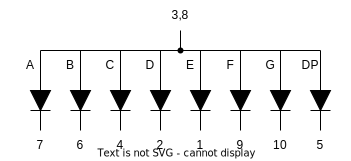
\includegraphics[width=15cm]{./img/image.png}
  \caption{メモリ確保エラー}
\end{figure}
メモリの確保が失敗した後にパソコンの画面が一瞬真っ黒になったため、そこで実験を終了した。
\section{付録:今回使用したプログラム}
\lstinputlisting[caption={hairetu.c}, label={lst:hairetu.c}]{211_kadai1.c}
\lstinputlisting[caption={ring.c}, label={lst:ring.c}]{211_kadai2.c}
\lstinputlisting[caption={list.c}, label={lst:list.c}]{211_kadai3.c}


\end{document}